\documentclass[utf8x, 12pt]{G7-32} 


% --------- -------- SETTINGS --------- --------

% --------- Настройки стиля ГОСТ 7-32 --------

% Гипертекстовое оглавление в PDF
\usepackage[
bookmarks=true, colorlinks=true, unicode=true,
urlcolor=black,linkcolor=black, anchorcolor=black,
citecolor=black, menucolor=black, filecolor=black,
]{hyperref}

\usepackage{graphicx}   % Пакет для включения рисунков
\DeclareGraphicsExtensions{.jpg,.pdf,.png}
\geometry{right=20mm}
\geometry{left=30mm}
\usepackage{enumerate}
\setcounter{tocdepth}{3} % Подробность оглавления


% --------- other settings --------
\usepackage{MnSymbol}
%\usepackage{simpsons}
% --------- -------- SETTINGS --------- --------



\begin{document}

\frontmatter 

% --------- -------- TITLE --------- --------

\begin{center} 

\large САНКТ-ПЕТЕРБУРГСИЙ ГОСУДАРСТВЕННЫЙ ПОЛИТЕХНИЧЕСКИЙ УНИВЕРСИТЕТ

\large Кафедра Компьютерных Систем и Программных Технологий \\[5.5cm] 

\huge ОТЧЕТ \\[0.6cm] % название работы, затем отступ 0,6см
\large по лабораторной работе №2\\
\large Тема: <<Система контроля версий Git>>\\
\large Дисциплина: <<Методы и средства защиты информации>>\\[3.7cm]

\end{center} 

\begin{flushright}
Выполнил: студент гр. 53501/2 \\
Пономарев М.A \\[1.2cm]


Преподаватель \\
Антонов А.П
\end{flushright}


\vfill 

\begin{center} 
\large Санкт-Петербург \\
2015
\end{center} 

\thispagestyle{empty}


% --------- -------- TITLE --------- --------

\thispagestyle{empty}
\setcounter{page}{0}
\tableofcontents
\clearpage
\mainmatter


\chapter{Задание}

\begin{enumerate}
	\item Изучить справку основных команд
	\item Получить содержимое репозитория
	\item Добавить новую папку и первый файл под контроль версий
	\item Зафиксировать изменения в локальном репозитории
	\item Внести изменения в файл и просмотреть различия
	\item Отменить локальные изменения
	\item Внести изменения в файл и просмотреть различия
	\item Зафиксировать изменения в локальном репозитории
	\item Зафиксировать изменения в центральном репозитории
	\item Получить изменения из центрального репозитория
	
	\medskip
	\item {\it Описать свои впечатления от работы}
\end{enumerate}



\chapter{Выполнение}


После изучения основных возможностей Git'a перейдём к выполнению задания:

\section{Создаём временный репозиторий}

Для изучения возможностей системы контроля версий создадим временный репозиторий на github под названием <<tempRepo>>. Далее, инициализируем пустой git репозиторий локально, добавляем файл README, для дальнейшей работы с репозиторием и создаём новую (главную) ветку разработки, фиксируем изменения в центральном репозитории.

\begin{figure}[hhh!]
	\begin{center}
		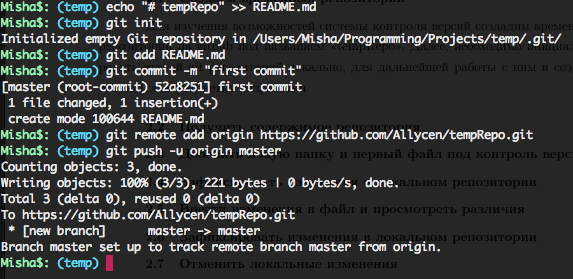
\includegraphics[width=12cm]{img/1}
	\end{center}
\end{figure}	


\section{Получить содержимое репозитория}

Для получения содержимого центрального репозитория используется команда <<git pull>> 

\begin{figure}[hhh!]
	\begin{center}
		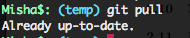
\includegraphics[width=4cm]{img/2}
	\end{center}
\end{figure}	

Система говорит нам, что локальный репозиторий не отличается от центрального.

\newpage

\section{Добавить новую папку и первый файл под контроль версий}

\begin{figure}[hhh!]
	\begin{center}
		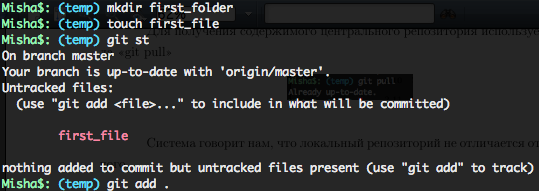
\includegraphics[width=12cm]{img/3}
	\end{center}
\end{figure}	


\section{Зафиксировать изменения в локальном репозитории}

\begin{figure}[hhh!]
	\begin{center}
		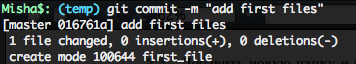
\includegraphics[width=8cm]{img/4}
	\end{center}
\end{figure}


\section{Внести изменения в файл и просмотреть различия}

\begin{figure}[hhh!]
	\begin{center}
		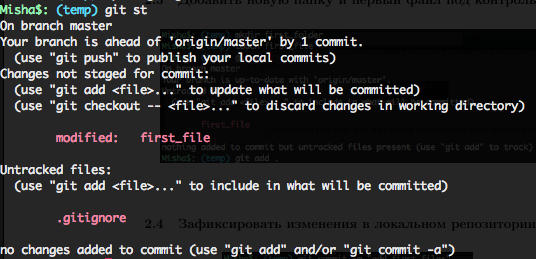
\includegraphics[width=12cm]{img/5}
	\end{center}
\end{figure}


\section{Зафиксировать изменения в локальном репозитории}

\begin{figure}[hhh!]
	\begin{center}
		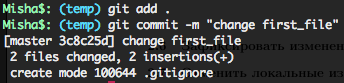
\includegraphics[width=8cm]{img/6}
	\end{center}
\end{figure}

\newpage

\section{Отменить локальные изменения}

\begin{figure}[hhh!]
	\begin{center}
		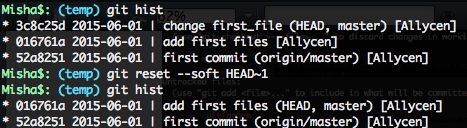
\includegraphics[width=12cm]{img/8}
	\end{center}
\end{figure}

\section{Внести изменения в файл и просмотреть различия}

\begin{figure}[hhh!]
	\begin{center}
		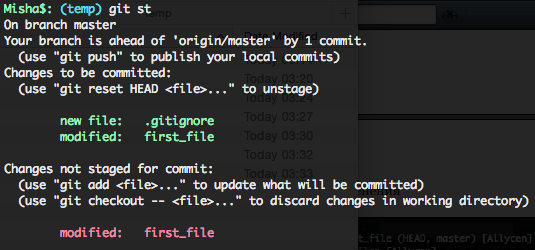
\includegraphics[width=12cm]{img/9}
	\end{center}
\end{figure}

Здесь очень важно, что когда мы применили команду <<reset --soft>>, мы всего лишь откатили последний коммит, но не обновление файла в системе контроля версий!

\section{Зафиксировать изменения в локальном репозитории}

\begin{figure}[hhh!]
	\begin{center}
		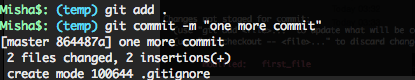
\includegraphics[width=12cm]{img/10}
	\end{center}
\end{figure}

\newpage

\section{Зафиксировать изменения в центральном репозитории}

\begin{figure}[hhh!]
	\begin{center}
		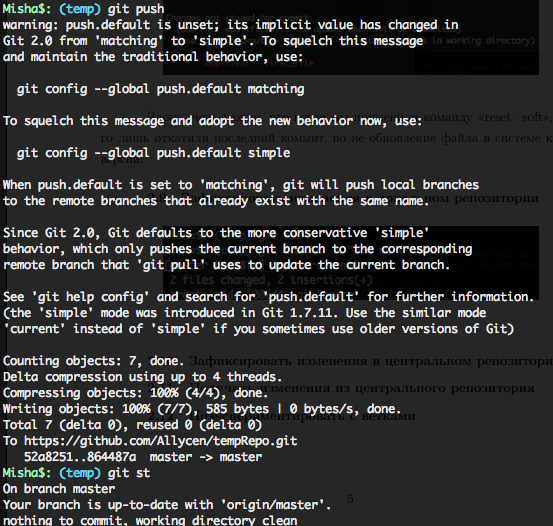
\includegraphics[width=12cm]{img/11}
	\end{center}
\end{figure}


\section{Получить изменения из центрального репозитория}

\begin{figure}[hhh!]
	\begin{center}
		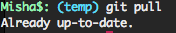
\includegraphics[width=4cm]{img/12}
	\end{center}
\end{figure}	



\end{document}
